\documentclass[11pt]{article}

% Paquetes esenciales
\usepackage[utf8]{inputenc}
\usepackage[spanish,es-tabla]{babel}
\usepackage{graphicx}
\usepackage{amssymb, amsmath}
\usepackage{textcomp}
\usepackage{geometry}
\usepackage{float}
\usepackage[bookmarks]{hyperref}
\usepackage[title, titletoc]{appendix}

% Paquetes opcionales
\usepackage{bookmark}
\usepackage{scrextend}
\bookmarksetup{numbered}
\usepackage[dvipsnames]{xcolor}
\usepackage{listings}
\makeatletter
\long\def\lst@maketitle#1#2{%
  \vskip\abovecaptionskip
    \bfseries #1: #2\par
  \vskip\belowcaptionskip}%
\makeatother
\lstset{%
    backgroundcolor=\color{gray!30},
    basicstyle=\ttfamily\small,
    basewidth=0.51em,
    tabsize=4,
    breaklines=true,
    showstringspaces=false,
    commentstyle=\color{black!60},
    stringstyle=\color{RedOrange},
    keywordstyle=\color{Maroon},
}
\definecolor{darkblue}{rgb}{0,0,.3}
\definecolor{darkgreen}{rgb}{0,.3,0}
\lstdefinelanguage{XML}
{
    morestring=[s][\color{black}]{>}{<},
    morestring=[b][\color{RedOrange}]",
    identifierstyle=\color{Maroon},
    keywordstyle=\color{darkgreen},
    morekeywords={xmlns,version,type,units,order,nps,variable},
}
\lstdefinelanguage{Python2}
{
    language=Python,
    morekeywords={as},
    otherkeywords={-,=}
}



% Título
\title{\textbf{KSource: Fuentes de partículas por \emph{Kernel Density Estimation}} \vspace{4mm} }
\author{
    \textbf{Osiris Inti Abbate} \vspace{2mm} \\
    \textit{Instituto Balseiro, UNCuyo - CNEA}
}
\date{\today}

\begin{document}

\maketitle

\begin{abstract}

KSource es una herramiente que asiste cálculos de blindajes por Monte Carlo, implementado una técnica de reducción de varianza. Procesa listas de partículas correspondientes a fuentes superficiales capturadas en posiciones intermedias de una simulación, estima su distribución por el método \emph{Kernel Density Estimation}, y produce nuevas partículas respetando la densidad estimada. Esto permite producir más partículas que las presentes en la lista original, sin repeticiones, favoreciendo la propagación de la radiación hacia la región de interés. Además, posibilita el acople de distintos códigos de cálculo.

\end{abstract}

%!TEX root = main.tex
\section{Introducción}

El método Monte Carlo es una técnica poderosa y ampliamente utilizada en el transporte de radiación. Su principal ventaja radica en la ausencia de aproximaciones sobre la distribución angular de los flujos de partículas, lo cual asegura una representación fiel incluso en problemas relativamente difíciles, como aquellos con absorbentes fuertes o propagación en vacío.

Un problema de transporte de radiación por Monte Carlo queda esencialmente definido por tres elementos principales:
\begin{itemize}
    \item Geometría: representación del sistema físico a modelar. Incluye los materiales involucrados y las condiciones de contorno.
    \item Fuente: región donde nacen las partículas, con una dada distribución energética, espacial y angular.
    \item Detector (\emph{tally}): resultado a obtener de la simulación, usualmente asociado al nivel de flujo o corriente en una región de interés. El cómputo del valor a reportar se realiza en base a las partículas que llegan al detector.
\end{itemize}

La principal dificultad del método Monte Carlo es el relativamente alto costo computacional requerido para obtener resultados confiables. La confiabilidad de un resultado se mide por su varianza estadística, la cual a su vez se relaciona con la cantidad de partículas utilizadas para calcularlo. Para resolver dicha problemática existen diferentes estrategias conocidas como \emph{técnicas de reducción de varianza}, las cuales buscan favorecer la propagación de la radiación hacia la región de interés, respetando la física del problema.

La herramienta KSource permite la implementación de una técnica de reducción de varianza, la cual se denominará método KSource. Los problemas de interés son entonces situaciones en las cuales no es posible alcanzar estadística suficiente en el detector en una única corrida, pues el costo computacional sería demasiado alto. Desde luego, siempre es posible determinar una superficie más cercana a la fuente en la cual sí es posible alcanzar buena estadística. Dicha situación se esquematiza en la Figura \ref{fig:esq_mc}, y es en la que se basa la aplicación del método KSource.

Continuando con el ejemplo de la Figura \ref{fig:esq_mc}, el método KSource consiste en registrar las partículas que atraviesan la superficie S1, obteniendo una lista de partículas (energía, posición, dirección) con estadística suficiente. Luego se utiliza dicha lista, también llamada lista de \emph{tracks}, para estimar la distribución de corriente en S1, y se utiliza dicha distribución estimada como fuente en una nueva simulación. La cantidad de partículas producidas en esta segunda etapa puede superar el tamaño de la lista original, mejorando la estadística en la región del detector y reduciendo la varianza del resultado. Todo este proceso se muestra en la Figura \ref{fig:esq_rv}. 

\begin{figure}[h!]
    \centering
    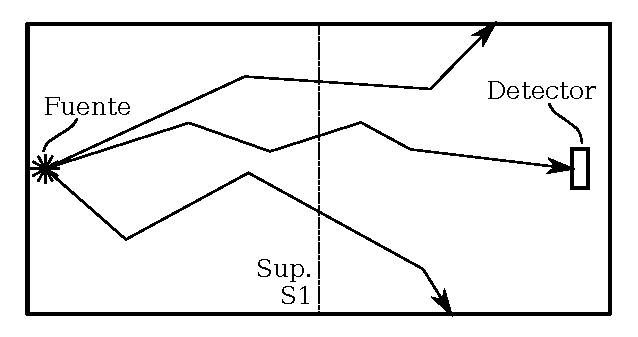
\includegraphics[width=.8\textwidth]{figs/esquema_simul.pdf}
    \caption{Esquema básico de una simulación por Monte Carlo. La superficie S1 permite la implementación de la técnica de reducción de varianza con la herramienta KSource.}
    \label{fig:esq_mc}
\end{figure}

\begin{figure}[htbp!]
    \centering
    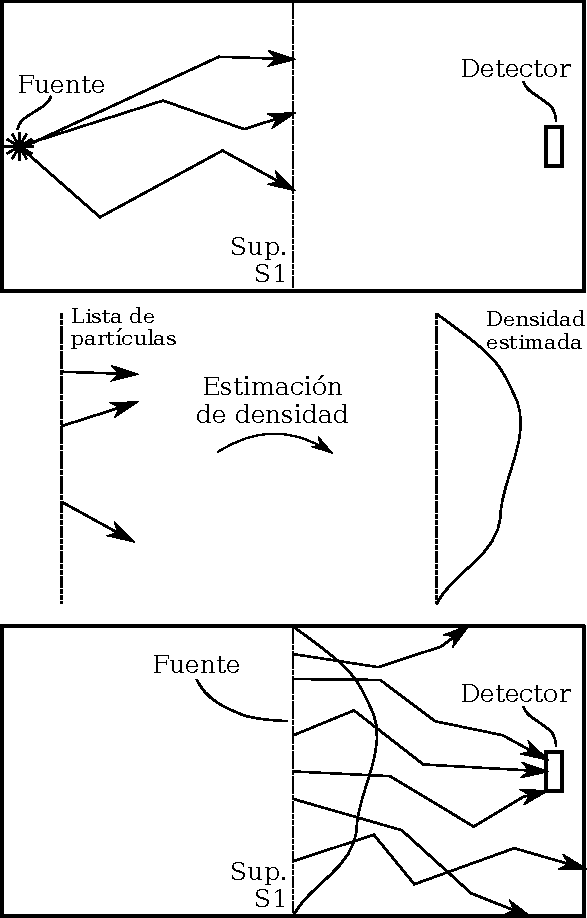
\includegraphics[width=.7\textwidth]{figs/esquema_redvar.pdf}
    \caption{Esquema de la implementación del método KSource. Se utiliza una lista de partículas registrada en una superficie intermedia para estimar su distribución, y utilizar esta última como fuente en una segunda simulación.}
    \label{fig:esq_rv}
\end{figure}


\subsection{\emph{Kernel Density Estimation}}
\label{subsec:kde}

El método empleado para la estimación de densidad es \emph{Kernel Density Estimation} (KDE). El mismo se basa en la siguiente expresión para la densidad estimada:

\begin{equation}
    \tilde{p}(x) = \frac{1}{N} \sum_{i=1}^N \frac{1}{|H|} K(H^{-1} (x-x^{(i)}))
    \label{eq:KDE}
\end{equation}
Donde:
\begin{itemize}
    \item $X = \{x^{(i)} \in \mathbb{R}^D\}_{1\leq i \leq N}$ es el conjunto de muestras que representa la lista de partículas.
    \item $\tilde{p}(x)$ es la densidad estimada en función del vector $x=(x_1,...,x_D)$.
    \item $K$ es el \emph{kernel} del método, que en KSource es la distribución normal (\emph{gaussiana}).
    \item $H$ es el ancho de banda (\emph{bandwidth}). En el caso más general considerado en KSource $H=H^{(i)}=(h_1^{(i)},...,h_D^{(i)})$ es un vector, el cual puede ser diferente para cada partícula. Cuando $H^{(i)}$ es diferente para cada partícula se dice que el método KDE es adaptativo.
\end{itemize}

Considerando el \emph{kernel} \emph{gaussiano} y el ancho de banda vector la expresión resulta:
\begin{equation}
    \label{eq:KDE-gauss}
    \tilde{p}(x) = \frac{1}{N (2\pi)^{D/2}} \sum_{i=1}^N \frac{1}{\prod_j h_j^{(i)}} exp\left(-\frac{1}{2} \sum_j \left(\frac{x_1-x_1^{(i)}}{h_1^{(i)}}\right)^2\right)
\end{equation}

El muestreo consiste en obtener nuevas muestras $\tilde{X} = \{\tilde{x}^{(i)} \in \mathbb{R}^D\}_{1\leq i \leq M}$ respetando la densidad estimada en \ref{eq:KDE}. Para el método KDE, la misma se realiza con el siguiente algoritmo:
\begin{itemize}
    \item Se toma un $x^{(i)} \in X$.
    \item Se obtiene la nueva muestra como $x = x^{(i)} + \Delta$, siendo $\Delta$ una perturbación aleatoria con la distribución del \emph{kernel} (\emph{gaussiana}) y los anchos de banda correspondientes a $x^{(i)}$.
\end{itemize}
Al repetir el muestreo, los $x^{(i)}$ se van tomando en orden tal como están en la lista de partículas. Cuando se llega al final, se vuelve al principio.

El ancho de banda es el parámetro más importante del método KDE. Para que la estimación de densidad tenga el mínimo error posible, los anchos de banda deben ser optimizados. Para ello KSource incluye tres métodos:
\begin{itemize}
    \item Regla de Silverman: Estima el ancho de banda óptimo únicamente en base a la cantidad de partículas en la lista, su dimensionalidad, y la desviación estándar $\sigma$ de cada variable. Es un método simple y rápido, aunque puede resultar en sobre-suavizado. Su fórmula es la siguiente:
    \begin{equation}
        h_{j,silv} = \left(\frac{4}{2+D}\right)^{\frac{1}{4+D}} N^{-\frac{1}{4+D}}
    \end{equation}  
    \item K Vecinos Más Cercanos (KNN): Calcula el ancho de banda para cada variable como la distancia al K-ésimo vecino más cercano, dentro de la lista de partículas, donde K es un parámetro fijado por el usuario. Es una técnica relativamente sencilla y rápida para obtener un ancho de banda variable (KDE adaptativo). 
    \item Validación Cruzada de Máxima Probabilidad (MLCV): Se basa en la maximización de la log-probabilidad media por validación cruzada, la cual funciona como factor de mérito de la estimación de densidad. Para ello se divide $X$ en dos conjuntos $X_{train}$ y $X_{test}$, y se calcula el factor de mérito como:
    \begin{equation}
        FM = \frac{1}{N_{test}} \sum_{X_{test}} \tilde{p}_{train}(x^{(i)}) 
    \end{equation}
    Donde $\tilde{p}_{train}$ es el modelo KDE construido con $X_{train}$.

    Se construye una grilla de anchos de banda partiendo de una semilla y una grilla de factores. Para cada ancho de banda se calcula el factor de mérito, y se toma el ancho de banda que lo maximiza. Es un método costoso computacionalmente, pero robusto ante diferentes distribuciones. Se obtiene la máxima optimización cuando se utiliza como semilla un ancho de banda obtenido por KNN.
\end{itemize}

El carácter multidimensional del ancho de banda, es decir que $h_j^{(i)}$ sea diferente para cada variable $j$, puede simplificarse a un caso unidimensional, donde $h_1^{(i)}=...=h_D^{(i)}$, mediante la normalización de datos. Usualmente, los anchos de banda para cada dimensión se toman como proporcionales a la desviación estándar de cada variable, es decir:
\begin{equation}
    h_j^{(i)} = h^{(i)} \sigma_j
\end{equation}
Introduciendo esta expresión en \ref{eq:KDE-gauss} se obtiene:
\begin{equation}
    \label{eq:DN}
    \tilde{p}(x) = \frac{1}{N (2\pi)^{D/2}} \sum_{i=1}^N \frac{1}{(h^{(i)})^D\prod_j \sigma_j} exp\left(-\frac{1}{2} \sum_j \left(\frac{x_1-x_1^{(i)}}{h^{(i)}\sigma_j}\right)^2\right)
    = \frac{1}{\prod_j \sigma_j} \tilde{p}_n(x_n)
\end{equation}
Donde $x_n=(\frac{x_1}{\sigma_1},...,\frac{x_D}{\sigma_D})$ es el vector normalizado, y $\tilde{p}_n$ es el modelo KDE construido con el conjunto de vectores normalizados, con anchos de banda $h^{(i)}$ unidimensionales.

La técnica consiste entonces en normalizar el conjunto $X$ de datos, empleando los $\sigma_j$ u otros factores de escaleo considerados apropiados, luego construir el modelo KDE normalizado $\tilde{p}_n(x_n)$, y finalmente obtener el modelo general de la ecuación \ref{eq:DN}. Los métodos de optimización de ancho de banda se aplican sobre el modelo normalizado.


\subsection[KDE en simulaciones Monte Carlo: ¿Cuándo y por qué es útil el método KDE?]{KDE en simulaciones Monte Carlo:\\¿Cuándo y por qué es útil el método KDE?}
\label{ssec:KDE-MC}

Considérese una simulación general por Monte Carlo con un único \emph{tally} $R$ y una fuente con distribución $S(x)$. En esta Subsección se analizará el impacto del error sistemático introducido por una fuente KDE sobre el valor de $R$, comparado con el muestreo directo de la lista de partículas, lo cual se denominará fuente de \emph{tracks}. Se utilizará para ello la propiedad de las distribuciones de Poisson según la cual, al contar en un \emph{tally} $n$ partículas, se tiene un error estadístico de $\sqrt{n}$.

Desde el punto de vista de la función importancia, también llamada flujo adjunto o función de Green \cite{AF}, el valor del \emph{tally} puede expresarse como:
\begin{equation}
    \label{eq:R}
    R = \int I(x) S(x) dx \approx I_0 \int_{\Omega} S(x) dx
\end{equation}
Donde $I$ es la función importancia, y la integración es sobre todo el espacio de fases. En la expresión aproximada se toma $I(x)$ como $I_0$ para $x \in \Omega$, y 0 afuera.

La fuente de \emph{tracks} puede expresarse como una suma de deltas de Dirac:
\begin{equation}
    S_t(x) = \frac{1}{N} \sum_i \delta\left(x-x^{(i)}\right)
\end{equation}

El valor del \emph{tally} resulta entonces:
\begin{equation}
    \label{eq:Rt}
    R_t = \frac{1}{N} \sum_i I(x^{(i)}) \approx \frac{n_{\Omega} I_0}{N}
\end{equation}
Donde $n_{\Omega}$ es la cantidad de partículas en la lista dentro de la región $\Omega$.

Por lo tanto, el error del \emph{tally} asociado a la fuente, en este caso, se puede estimar como:
\begin{equation}
    \frac{\Delta R_t^{sist}}{R_t} = \frac{1}{\sqrt{n_{\Omega}}}
\end{equation}

Para la fuente KDE, por simplicidad, se supondrá un ancho de banda único $h$, ya optimizado. Para la estimación de $R$ con dicha fuente se distinguirán dos situaciones:
\begin{itemize}
    \item $\mu(\Omega) >> h^D$
    \item $\mu(\Omega) << h^D$
\end{itemize}
Donde $\mu(\Omega)$ es la medida de la región $\Omega$.

En el primer caso, al ser el ancho de banda mucho menor a la longitud característica de $\Omega$, el resultado en el \emph{tally} resultará muy similar al caso con fuente de \emph{tracks}. También será similar el error asociado a la fuente, salvo por un \emph{bias} dependiente del valor medio de la pendiente de la distribución de fuente en la frontera de $\Omega$.

En este caso se puede concluir que el método KDE no resulta de gran utilidad, ya que no mejora el error del \emph{tally} asociado a la fuente. Resulta más apropiado utilizar la fuente de \emph{tracks}, si es necesario muestreando varias veces cada partícula en la lista, para reducir el error estadístico de la simulación.

En el segundo caso, al ser el ancho de banda mucho mayor a la longitud característica de $\Omega$, se puede suponer a $S_{KDE}(x)$ como lineal dentro de $\Omega$, y aproximar $R$ como:
\begin{equation}
    R_{KDE} = I_0 \mu(\Omega) S_{KDE}(x_0)
\end{equation}
Donde $S_{KDE}$ es la distribución de la fuente KDE, y $x_0$ es un vector de fase dentro de $\Omega$.

El error de $R$ asociado a la fuente, en este caso, se obtiene directamente del error puntual del método KDE. El mismo se compone de un error estadístico, que depende de la cantidad de partículas usadas en la estimación, y un \emph{bias} por el suavizado \cite{NP}.
\begin{equation}
    \frac{\Delta R_{KDE}^{sist}}{R_{KDE}} = \frac{\sqrt{r}}{\sqrt{n_h}} + bias(x_0)
\end{equation}
Donde $n_h$ es la cantidad de partículas dentro de una hiper-esfera de radio $h$ centrada en $x_0$, y $r$ es la denominada rugosidad del \emph{kernel}, que vale $1/2\sqrt{\pi}$ para el \emph{kernel} \emph{gaussiano}. Para otros \emph{kernels} siempre es del orden de 1.

Es en este caso en el que el método KDE puede resultar útil, reduciendo el error en el \emph{tally} asociado a la fuente. Debido a que $\mu(\Omega) << h^D$, se tiene que $n_{\Omega} << n_h$, y por lo tanto $1/\sqrt{n_{\Omega}} >> 1/\sqrt{n_h}$. Es decir que el método KDE reduce significativamente el error de $R$ asociado al error estadístico de la fuente, aunque a costa de un error adicional asociado al \emph{bias}. Si bien no es posible asegurar de forma general el resultado de dicho balance, es de esperar que, gracias a la optimización del ancho de banda, una mejora sea probable.

En conclusión, las situaciones en la que el método KDE resulta más útil son aquellas en las que la región de la fuente que afecta el \emph{tally} es pequeña, con pocas partículas en su interior, y en particular con distancias características menores al ancho de banda optimizado. Al haber pocas partículas en la región de fuente ``observada'' por el \emph{tally}, el error asociado a una fuente de \emph{tracks} es grande, y el suavizado que realiza el método KDE, teniendo en cuenta un mayor número de partículas, resulta beneficioso. Estas situaciones pueden relacionarse con problemas de propagación en vacío, donde existen pocos caminos por los cuales las partículas pueden llegar de la fuente a la región de interés, en contraposición con los problemas de moderación.

La herramienta KSource, a pesar de estar esencialmente orientada a fuentes KDE, también permite implementar fuentes de \emph{tracks}, y en ambos casos facilita el acople entre códigos Monte Carlo.


%!TEX root = main.tex
\section{Contenidos del paquete KDSource}

La herramienta KDSource cuenta con los siguiente componentes:
\begin{itemize}
	\item Biblioteca en Python, para estimación de densidad. Aquí se encuentras las herramientas necesarias para crear y optimizar una fuente KDSource en base a una lista de partículas. Se puede además analizar su estadística, generar gráficos de las distribuciones, y exportar la fuente creada, para su uso en los otros componentes de KDSource.
	\item Biblioteca en C, para muestreo. Aquí se encuentras las herramientas necesarias para muestrear nuevas partículas, en base a una fuente KDSource previamente creada.
	\item Aplicación de línea de comando. Permite ejecutar un re-muestreo de partículas, en base a una fuente KDSource previamente creada, obteniéndose una lista de partículas de longitud arbitraria. También permite acceder de forma simple a otras utilidades incuidas en el paquete.
	\item Plantillas y archivos útiles. Facilitan las operaciones más usuales con el paquete KDSource. Se incluyen archivos Jupyter Notebook con las operaciones más usuales de la biblioteca de Python, así como \emph{scripts} y otros componentes para ejecutar algunos códigos Monte Carlo en acople con KDSource.
\end{itemize}

En la Sección \ref{sec:libs} se describen los principales objetos definidos en las librerías, mediante los cuales se modelan y manipulan las fuentes KDE. En los Apéndices  \ref{ap:CLI}, \ref{ap:Python} y \ref{ap:C} se presenta la documentación detallada de la aplicación de línea de comando y de las librerías. Por otra parte, en la Sección \ref{sec:FT} se describe el flujo de trabajo requerido para emplear la herramienta KDSource en una simulación Monte Carlo.


\section{El formato de fuente KDSource}
\label{sec:libs}

La herramienta KDSource cuenta con librerías para modelar fuentes distribucionales de partículas en Python y C. En ambos casos se define la estructura \verb|KDSource|, la cual a su vez posee dos subestructuras: \verb|PList| y \verb|Geometry|. Éstas modelan los dos componentes fundamentales de una fuente KDSource: La lista de partículas y su geometría. En Python, la técnica KDE se implementa a través de la librería \verb|KDEpy| \cite{KDEpy}.

\subsection{Listas de partículas}

Las listas de partículas utilizadas en KDSource utilizan el formato MCPL \cite{MCPL}. El mismo permite la comunicación con los siguientes códigos Monte Carlo:
\begin{itemize}
	\item MCNP
	\item PHITS
	\item McStas
	\item GEANT4
	\item TRIPOLI-4
\end{itemize}
Esto quiere decir que es posible convertir las listas de partículas registradas por cualquiera de estos códigos a MCPL, y viceversa. El \emph{software} asociado al formato MCPL está incluido en la distribución de KDSource, incluyendo funcionalidades extra con respecto a la distribución original, como la posibilidad de comunicación con TRIPOLI-4.

La estructura \verb|PList| empleada en las librerías administra la comunicación con el archivo MCPL. Además de la lectura y escritura, se incluye la posibilidad de aplicar una traslación y rotación a las partículas inmediatamente despues de leerlas, lo cual puede ser útil al acoplar simulaciones con distinto sistema de referencia.

\subsection{Geometría}

A pesar de su nombre, la estructura \verb|Geometry| no sólo administra la geometría de fuente, sino también la manera en que se debe tratar la energía y dirección de las partículas. El objetivo fundamental de esta estructura es convertir el conjunto de parámetros que definen una partícula, es decir energía, posición y dirección, a un vector de parametrización (variables parametrizadas), más adecuado para la aplicación del método KDE. Dicho vector es el que se utilizará como $x$ en las expresiones de la Subsección \ref{subsec:kde}.

Para dar versatilidad al tratamiento energético, espacial y angular deseado, la estructura \verb|Geometry| posee a su vez un conjunto de subestructuras de tipo \verb|Metric|. Usualmente se cuenta con tres de éstas: una para la energía, una para la posición, y una para la dirección. Cada \verb|Metric| define la métrica con la que se tratará cada conjunto de variables. Los objetos \verb|Metric| pueden elegirse del conjunto de métricas implementadas:
\begin{itemize}
	\item \verb|Energy|: tratamiento simple de la energía, sin transformaciones.
	\item \verb|Lethargy|: emplear letargía en lugar de energía.
	\item \verb|Vol|: tratamiento espacial volumétrico.
	\item \verb|SurfXY|: tratamiento espacial plano en XY.
	\item \verb|Guide|: geometría de guía de sección rectangular, con tratamiento de los ángulos basado en la superficie de cada espejo.
	\item \verb|Isotrop|: tratamiento simple de la dirección, basado en el versor unitario de dirección.
	\item \verb|Polar|: tratamiento de la dirección en base a los ángulo $\theta$ (distancia angular a la dirección $\hat{z}$) y $\phi$ (acimut medido desde la dirección $\hat{x}$).
	\item \verb|PolarMu|: igual a \verb|Polar|, pero con $\mu = cos(\theta)$ en lugar de $\theta$.
\end{itemize}

En la biblioteca de Python, la función principal tanto de \verb|Geometry| como de \verb|Metric| es la de transformar las partículas en el formato de partícula de MCPL al vector de parametrización, en formato de \verb|numpy.array|. Esto se logra a través de las funciones \verb|transform| e \verb|inverse_transform|.

En la biblioteca de C, por su parte, considerando que ésta se enfoca en el muestreo de partículas, lo cual se logra mediante la perturbación (ver \ref{subsec:kde}), la función principal de \verb|Geometry| y \verb|Metric| es la de perturbar partículas, respetando la métrica correspondiente y con los anchos de banda provistos. Esto se logra con las funciones \verb|[MetricName]_perturb|, donde \verb|[MetricName]| se debe reemplazar por el nombre de cada métrica.

El objeto \verb|Geometry| también incluye (opcionalmente) una traslación y rotación espacial. Esto permite modelar fuentes ubicadas en dististas posiciones y con distintas orientaciones con respecto al sistema de coordenadas. Por ejemplo, permite modelar una fuente en el plano YZ mediante la métrica \verb|SurfXY|, a través de una rotación de 90 grados en el eje Y. 

\subsection{Archivos de parámetros XML}

Las fuentes creadas en Python, luego de la optimización, pueden guardarse en un archivo de parámetros en formato XML. En el mismo se registran los parámetros que definen las estructuras \verb|PList| y \verb|Geometry| que componen la fuente \verb|KDSource|, así como el \emph{path} al archivo MCPL a utilizar. Este archivo de parámetros puede luego utilizarse para reconstruir la fuente mediante la biblioteca en C, o bien para re-muestrear directamente mediante la aplicación de línea de comando.

Si el ancho de banda del modelo es constante, su valor también se guarda en el mismo archivo XML. Si, por el contrario, el ancho de banda es variable (KDE adaptativo), es decir que se representa con un \emph{array} de un valor por partícula, el mismo se guarda en un archivo separado, en formato binario. Para maximizar el ahorro de memoria, especialmente importante en listas de partículas largas, se utiliza el formato de punto flotante de simple presición (32 bits), sin separación entre valores.


\section{Flujo de trabajo}
\label{sec:FT}

El esquema del flujo de trabajo típico con la herramienta KDSource se esquematiza en la Figura \ref{fig:flujo}. Se parte de una lista de partículas inicial, la cual puede, o no, haber sido creada en una simulación anterior, y luego se ejecuta cierto número de simulaciones Monte Carlo. Cada una de ellas emplea una fuente de partículas KDSource basada en la lista de partículas registrada inmediatamente antes, y registra una nueva lista de partículas para la etapa siguiente. Dependiendo del problema, pueden obtenerse resultados útiles en todas las simulaciones (por ejemplo, al construir un mapa de dosis), o bien sólo en la última (por ejemplo, al calcular el flujo a la salida de un haz). Cada simulación cubre una región de la geometría modelada progresivamente más lejana a la fuente inicial, alcanzando distancias que no serían alcanzables en una sola corrida.

\begin{figure}[b!]
	\centering
	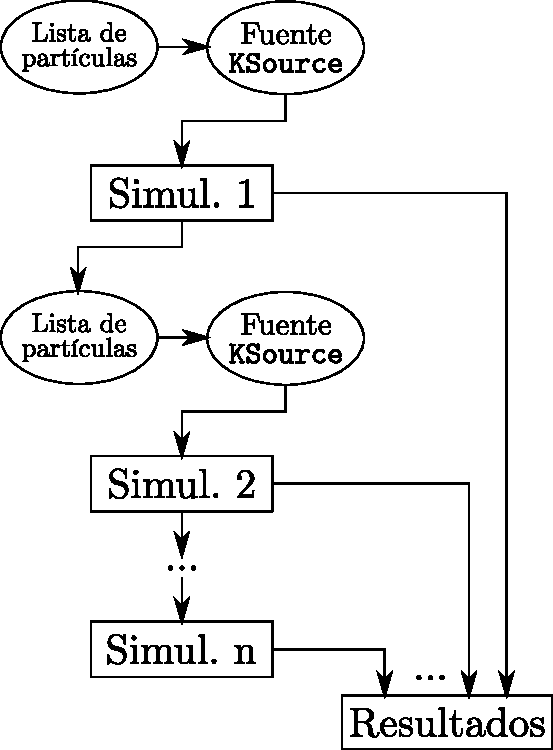
\includegraphics[width=.7\textwidth]{figs/flujo_trabajo.pdf}
	\caption{Esquema del flujo de trabajo típico.}
	\label{fig:flujo}
\end{figure}

Cada construcción de una fuente KDSource en base a una lista de partículas se realiza mediante la API en Python, y culmina al exportar un archivo de parámetros XML. Se provee una plantilla con el código requerido para dicha tarea en el archivo \verb|preproc_tracks.ipynb|.

Es recomendable ejecutar dos veces cada etapa de simulación, una de ellas utilizando la fuente KDE de la manera usual, y en la otra muestreando partículas directamente de la lista de \emph{tracks}. Esto puede lograrse de forma simple fijando el argumento \verb|use_kde=0| en la función de muestreo, empleando la misma fuente \verb|KDSource|. El objetivo de dicha repetición del cálculo es verificar la compatibilidad de los resultados obtenidos con ambas fuentes.

De acuerdo a lo explicado en la Subsección \ref{ssec:KDE-MC}, las fuentes de \emph{tracks} pueden añadir mayor ``ruido'' a la simulación, pero no introducen ningún sesgo. Las fuentes KDE, gracias a su mejor estadística, permiten obtener resultados más detallados en zonas lejanas a la fuente, y más suaves, pero corren el riesgo de introducir errores sistemáticos debidos al sesgo de suavizado. Si los resultados que es posible obtener con ambas simulaciones (cercanos a la fuente) coinciden con ambas fuentes, puede considerarse que el sesgo de la fuente KDE es suficientemente bajo, y ``confiar'' en los resultados más lejanos.


\subsection{Simulaciones con McStas y TRIPOLI-4}

Si el código utilizado fuera McStas o TRIPOLI-4, se incluyen además archivos plantilla para facilitar las tareas de interpretación de los resultados de las simulaciones. El archivo \verb|postproc.ipynb| permite colectar los principales resultados, para su registro en una planilla de cálculo. Por otra parte, el archivo \verb|doseplots.ipynb| facilita la creación de gráficos de los mapas de dosis registrados en TRIPOLI-4, utilizando un módulo de Python incluido para tal fin.


\subsection{Acople entre óptica neutrónica y transporte con McStas}

Entre los componentes de McStas incluidos en el paquete KDSource se encuentra\linebreak \verb|Guide_shielding|, mediante el cual es posible efectuar cálculos de blindaje en la perfiferia de guías neutrónicas, respetando la física correspondiente a la óptica neutrónica. Esto se logra a través de un acople en un solo sentido (\emph{one-way coupling}) entre McStas y un código de transporte de radiación, como MCNP, PHITS o TRIPOLI.

El componente \verb|Guide_shielding|, en una simulación de McStas, funciona de igual manera que otros componentes que simulan guías neutrónicas. En particular modela guías de sección rectangular, con posibilidad de curvatura (similar a \verb|Bender|). La diferencia radica en que, al mismo tiempo que propaga los neutrones en su interior, registra en un archivo MCPL los escapes a través de sus espejos. Es decir que por cada reflexión, se registra la energía, posición y dirección del neutrón incidente, y el peso estadístico de la fracción no reflejada. En McStas la simulación continúa con la porción reflejada.

La lista de partículas obtenida representa una fuente superficial de neutrones escapando a través de los espejos de la guía. Dicha fuente no es plana, sino que tiene forma de tubo, posiblemente curvado, de sección rectangular, y es la causante de la presencia de radiación en la periferia de la guía, la cual debe ser blindada. Este archivo MCPL debe utilizarse entonces para construir una fuente KDE mediante la herramienta KDSource, con ayuda del archivo plantilla \verb|preproc_tracks.ipynb|, y emplear esta última en un cálculo de blindajes de la región que rodea a la guía, tipicamente un búnker o \emph{hall}.

El componente \verb|Guide_shielding| registra, además, las partículas \emph{gamma} emitidas por absorciones en el níquel o titanio de los espejos, de acuerdo a las relaciones presentadas en \cite{abs}. Las absorciones se descuentan del peso estadístico de los neutrones transmitidos, por lo que no afectan las curvas de reflectividad. Por la alta energía de los fotones \emph{prompt} del níquel, el correcto modelado de dicho fenómeno es importante para no subestimar la dosis \emph{gamma} alrededor de la guía, especialmente ante flujos neutrónicos con alta componente térmica y fría. Los fotones generados, con energías obtenidas de los espectros de emisión y direcciones isotrópicamente aleatorias, son registrados en otro archivo MCPL, el cual debe ser utilizado para generar una fuente KDE para un cálculo de blindajes, del mismo modo que con la fuente de escapes neutrónicos.


\subsection{Fuentes de activación con TRIPOLI-4 (u otros códigos)}

Una fuente de activación es una fuente de radiación gamma proveniente del decaimiento radiactivo de nucleidos inestables presentes en un material, producidos mediante reacciones nucleares (activación neutrónica). Dicha fuente no es superficial, sino volumétrica. Desde luego, la herramienta KDSource es capaz de modelar este tipo de fuentes a través de la técnica KDE, pero, como siempre, necesita para ello una lista de partículas. En este caso dicha lista debe contener las propiedades de los fotones al momento de cada decaimiento, cuya interpretación es la siguiente:
\begin{itemize}
	\item Energía: Tiene valores discretos, los cuales, junto con sus frecuencias de ocurrencia, conforman el denominado espectro de decaimiento.
	\item Posición: Se corresponden con los puntos en los que ocurrieron las reacciones de activación.
	\item Dirección: Cada gamma de activación tiene una dirección isotrópicamente aleatoria.
\end{itemize}

Esto quiere decir que, de contarse con una lista de fotones de activación, puede procederse a contruir una fuente KDE con las herramientas descritas anteriormente, en particular con la ayuda del archivo plantilla \verb|preproc_tracks.ipynb|. Debe tenerse la precaución de fijar en cero los anchos de banda en energía, para respetar el carácter discreto del espectro de decaimiento.

Sin embargo, el modo más usual de registrar la activación en materiales es a través de \emph{tallies} volumétricos. En conjunto con el espectro de decaimiento, es posible utilizar dichos \emph{tallies} para crear una lista de gammas de decaimiento, y luego aplicar las herramientas de KDSource. En particular, para el código TRIPOLI-4, la API en Python de KDSource cuenta con un módulo que permite realizar de forma sencilla la conversión de \emph{tally} a lista de \emph{tracks}, mediante la clase \verb|T4Tally|. Además, el archivo plantilla \verb|preproc_tally.ipynb| cuenta con el conjunto de operaciones necesarias para construir una fuente KDE, en base a un \emph{tally} de activación de TRIPOLI-4 y un espectro de decaimiento. 


\begin{appendices}
    %!TEX root = main.tex
\section{Descripción del formato de archivo de parámetros XML}

Un archivo de parámetros XML es el método por el cual se puede almacenar una fuente KDE en el disco. Usualmente dicho archivo es generado mediante la API en Python, luego de la optimización del ancho de banda. Este formato sirve además como método de comunicación entre los distintos componentes de KDSource, ya que puede utilizarse para reconstruir una fuente tanto en Python como en C, y para aplicar re-muestreo por línea de comando.

Como se muestra en el ejemplo del Listing \ref{lst:xmlfile}, un archivo de parámetros posee la siguiente información:
\begin{itemize}
	\item Corriente total de la fuente, en unidades $[1/s]$.
	\item \verb|PList|: Lista de partículas.
	\begin{itemize}
		\item Tipo de partícula global.
		\item Archivo MCPL con la lista de partículas.
		\item Traslación (opcional).
		\item Rotación (opcional).
		\item Transformación $(x,y,z)\rightarrow (y,z,x)$ (opcional).
	\end{itemize}
	\item \verb|Geom|: Geometría y tratamiento de variables. El orden indica la cantidad de sub-métricas.
	\begin{itemize}
		\item Submétricas. Para cada una, además de su nombre, se indica:
		\begin{itemize}
			\item Dimensionalidad.
			\item Parámetros (específicos para cada métrica).
		\end{itemize}
		\item Traslación (opcional).
		\item Rotación (opcional).
	\end{itemize}
	\item Factores de escaleo para cada variable de parametrización.
	\item Ancho de banda. Si es constante (\verb|variable="0"|) se indica su valor, mientras que si es adaptativo (\verb|variable="1"|) se indica el \emph{path} del archivo conteniendo la lista de valores. Dicho archivo debe poseer una secuencia de valores en formato binario de punto flotante de simple precisión (32 bits), sin separación, de la misma longitud que la lista de partículas en el archivo MCPL.
\end{itemize}

\begin{lstlisting}[language=XML, label={lst:xmlfile}, caption=Ejemplo de archivo de parámetros XML.]
<?xml version="1.0" ?>
<KDSource>
	<J units="1/s">1.0</J>
	<PList>
		<pt>n</pt>
		<mcplname>/path/to/mcplfile.mcpl.gz</mcplname>
		<trasl>  0.   0. -10.</trasl>
		<rot/>
		<x2z>0</x2z>
	</PList>
	<Geom order="3">
		<Lethargy>
			<dim>1</dim>
			<params nps="1">10.0</params>
		</Lethargy>
		<SurfXY>
			<dim>2</dim>
			<params nps="5">-50. 50. -50. 50. 0.</params>
		</SurfXY>
		<PolarMu>
			<dim>2</dim>
			<params nps="0"/>
		</PolarMu>
		<trasl>10.  0. 50.</trasl>
		<rot>0.         3.14159265 0.        </rot>
	</Geom>
	<scaling>2.2339 14.1445 10.0147 0.2362 103.6779</scaling>
	<BW variable="1">/path/to/bwfile</BW>
</KDSource>
\end{lstlisting}




\section{Documentación de aplicación \texttt{kdtool}}
\label{ap:CLI}

La aplicación de linea de comando de KDSource se accede a través del comando \verb|kdtool|. Sus instrucciones de uso se pueden obtener mediante el argumento \verb|--help|, y se muestran en el Listing \ref{lst:kdtool}.

\begin{lstlisting}[label={lst:kdtool}, caption=Instrucciones de uso del comando \texttt{kdtool} (output de ``\texttt{kdtool --help}'').]
Usage: kdtool [options]

KDSource is a Monte Carlo calculations assistance tool. It implements particles
density estimation and sampling by means of Kernel Density Estimation method.

Options:
	resample:   Resample particles based on a kdsource XML file.
	templates:  Copy templates for Monte Carlo calculations.
	beamtest:   Test source with simple beam calculation.
	[Any MCPL command]
	-h, --help: Display usage instructions.
\end{lstlisting}

La opción \verb|resample| de \verb|kdtool| permite generar nuevas muestras en base a un modelo KDSource guardado en un archivo de parámetros XML. Sus instrucciones de uso se pueden obtener mediante el argumento \verb|--help|, y se muestran en el Listing \ref{lst:resample}.

\begin{lstlisting}[label={lst:resample}, caption=Instrucciones de uso del comando \texttt{kdtool resample} (output de ``\texttt{kdtool resample --help}'').]
Usage: kdtool resample sourcefile [options]

Resample particles from source defined in XML file sourcefile, and save them in
a MCPL file.

Options:
	-o outfile: Name of MCPL file with new samples
	            (default: \"resampled.mcpl\").
	-n N:       Number of new samples (default: 1E5).
	-h, --help: Display usage instructions.
\end{lstlisting}

La opción \verb|templates| de \verb|kdtool| permite copiar los archivos plantilla (Jupyter Notebooks) de las operaciones más usuales con la API de Python al directorio de trabajo. Además, opcionalmente, permite copiar plantillas para ejecutar McStas o TRIPOLI-4 en acople con KDSource. Sus instrucciones de uso se pueden obtener mediante el argumento \verb|--help|, y se muestran en el Listing \ref{lst:templates}.

\begin{lstlisting}[label={lst:templates}, caption=Instrucciones de uso del comando \texttt{kdtool templates} (output de ``\texttt{kdtool templates --help}'').]
Usage: kdtool templates dest [options]

Copy to dest templates for KDSource usage in Python, or for interacting with
Monte Carlo codes.

Options:
	--mcstas:   Copy templates for using McStas.
	--tripoli:  Copy templates for using TRIPOLI-4.
	--all:      Copy all templates.
	-h, --help: Display usage instructions.
\end{lstlisting}

La opción \verb|beamtest| permite evaluar la validez de la fuente KDE en un cálculo de haces, comparando su funcionamiento con la fuente de \emph{tracks} (muestreo directo de partículas de la lista). Su uso está orientado a fuentes planas de neutrones, y la comparación consiste en una simulación en la cual se propagan las partículas de fuente hasta un colimador rectangular, donde se mide la corriente. Dicha simulación se ejecuta dos veces, una con la fuente KDE y una muestreando las partículas directamente de la lista, y los resultados se almacenan en un documento de texto. Es posible configurar la posición y tamaño del colimador rectangular, para evaluar la concordancia entre ambas fuentes en distintos casos. Sus instrucciones de uso se pueden obtener mediante el argumento \verb|--help|, y se muestran en el Listing \ref{lst:beamtest}.

\begin{lstlisting}[label={lst:beamtest}, caption=Instrucciones de uso del comando \texttt{kdtool beamtest} (output de ``\texttt{kdtool beamtest --help}'').]
Usage: kdtool beamtest sourcefile [options]

Executes a simple simulation with source defined in XML file sourcefile, in
which calculates the number of particles passing thru a rectangular collimator.
The simulation is repeated using the particle list directly as source, to
compare the results.

Results are computed for 4 energy groups, and stored in a results file which
can be imported from a spreadsheet.

This tool is designed to be used with flat neutron sources with particles
propagating towards z direction.

Options:
	-n N:           Number of source particles (default: 1E6).
	-o results:     Name of file to store results.
	-xwidth value:  Width of the collimator, in cm (default: 7).
	-yheight value: Height of the collimator, in cm (default: 20).
	-z value:       Position of the collimator along z axis, in cm
	                (default: 500).
	-xshift:        Horizontal shift of the center of the collimator,
	                in cm (default: 0)
	-yshift:        Vertical shift of the center of the collimator,
	                in cm (default: 0)
	-h, --help:     Display usage instructions.
\end{lstlisting}

Por último, el comando \verb|kdtool| permite acceder a cualquiera de las aplicaciones de línea de comando de MCPL, en su versión extendida incluida en el paquete KDSource.



\section{Documentación de API en Python}
\label{ap:Python}

La API en Python de KDSource, denominada \verb|kdsource|, se compone de los siguientes módulos:
\begin{itemize}
	\item \verb|kdsource.py|: Módulo para el objeto \verb|KDSource|, que representa una fuente KDE.
	\item \verb|kde.py|: Módulo para métodos de selección de ancho de banda, para la librería \verb|KDEpy|.
	\item \verb|plist.py|: Módulo para el objeto \verb|PList|, y operaciones sobre listas de partículas.
	\item \verb|geom.py|: Módulo para el objeto \verb|Geometry|, la clase abstracta \verb|Metric|, y todas sus implementaciones heredadas.
	\item \verb|stats.py|: Módulo para análisis estadístico de listas de partículas, mediante el objeto \verb|Stats|.
	\item \verb|summary.py|: Módulo para colectar los principales resultados de simulaciones Monte Carlo, mediante el objeto \verb|Summary|.
	\item \verb|tally.py|: Módulo para lectura, gráficos, y conversión a lista de partículas, de \emph{tallies} de TRIPOLI-4, mediante el objeto \verb|T4Tally|.
	\item \verb|utils.py|: Utilidades generales.
\end{itemize}

Todas las funcionalidades de los módulos mencionados se encuentran presentes en el \emph{namespace} principal de la librería \verb|kdsource|.


\subsection{Ejemplo de uso}

\begin{lstlisting}[language=Python2, label={lst:exa}, caption=Ejemplo básico de uso de API en Python.]
import kdsource as kds

# Define particle list
plist = kds.PList("surfsource", readformat="ssw")
# Define geometry
geom = kds.GeomFlat()
# Create KDSource
s = kds.KDSource(plist, geom, bw="mlcv")

# Fit KDSource
s.fit(N=1E5)

# Save in XML file
s.save("source.xml")
\end{lstlisting}

En el Listing \ref{lst:exa} se muestra un ejemplo básico de uso. Las principales etapas son:
\begin{itemize}
	\item Creación de objeto \verb|KDSource| en base a objetos \verb|PList| y \verb|Geometry|.
	\item Ajuste de anchos de banda.
	\item Gráficos de distribuciones.
	\item Guardado de la fuente en archivo XML.
\end{itemize}

En los archivos plantilla (disponibles mediante ``\verb|kdtool templates .|'') se muestran más ejemplos de uso de los distintos módulos de KDSource.


\subsection{Módulo \texttt{kdsource}}

Este módulo se centra en la clase \verb|KDSource|, que modela una fuente de partículas KDE. Para su creación se debe contar previamente con objetos \verb|PList| y \verb|Geometry|. Mediante un modelo \verb|KDSource| se puede aplicar el método KDE sobre una lista de partículas, optimizar el ancho de banda, generar gráficos de las distribuciones estimadas, y guardar el modelo en un archivo XML, para su posterior uso con la misma u otras APIs.

El objeto \verb|KDSource| sirve como \emph{wrapper} de un modelo KDE de la librería \verb|KDEpy|, el cual guarda en el parámetro \verb|kde|. Es posible modificar manualmente el ancho de banda modificando el parámetro \verb|bw| de dicho objeto. Además \verb|KDSource| posee un parámetro \verb|scaling|, el cual contiene los factores de normalización para cada variable (ver \ref{subsec:kde}).

En el Listing \ref{lst:exa} se muestra un ejemplo de uso básico del objeto KDSource, mientras que en el Listing \ref{lst:exa-plot} se muestra el uso de las funciones de gráficos. Es posible realizar gráficos tanto 1D como 2D, y para cada uno de ellos existen 2 posibilidades:
\begin{itemize}
	\item Gráficos integrados: Se grafica la densidad en función de 1 ó 2 variables parametrizadas, integrando sobre las demás (en un rango finito o en todo su dominio). Este es el caso de \verb|plot_integr|, \verb|plot_E| y \verb|plot2D_integr|. Es el método de graficación recomendado. La función \verb|plot_E| grafica el espectro en función de la energía independientemente de la parametrización elegida. 
	\item Gráficos puntuales: Se grafica la densidad conjunta en función de 1 ó 2 variables no parametrizadas. Este es el caso de \verb|plot_point| y \verb|plot2D_point|.
\end{itemize}

\begin{lstlisting}[language=Python2, label={lst:exa-plot}, caption=Ejemplo de gráficos de distribuciones estimadas.]
# Energy plot
EE = np.logspace(-9,1,50)
fig,[scores,errs] = s.plot_E(EE)
plt.show()

# Theta plot
tt = np.linspace(0,180,50)
fig,[scores,errs] = s.plot_integr("theta", tt)
plt.show()

# XY plot of epithermal neutrons
umin = 3  # Minimum lethargy
umax = 16 # Maximum lethargy
# Vector of min and max vals (parametrized)
#      [u   , x     , y     , theta, phi]
vec0 = [umin,-np.inf,-np.inf, 0    ,-180]
vec1 = [umax, np.inf, np.inf, 180  , 180]
xx = np.linspace(-10,10,30)
yy = np.linspace(-10,10,30)
s.plot2D_integr(["x,y"], [xx,yy], vec0=vec0, vec1=vec1)
plt.show()

# XY plot at fixed energy and angle
# Vector of fixed values (non parametrized)
#       [E   , x, y, z, dx, dy, dz]
part0 = [1E-3, 0, 0, 0, 0 , 0 , 1 ]
xx = np.linspace(-10,10,30)
yy = np.linspace(-10,10,30)
s.plot2D_point(["x,y"], [xx,yy], part0=part0)
plt.show()
\end{lstlisting}


\subsection{Módulo \texttt{kde}}

Este módulo contiene métodos de selección de ancho de banda que complementan la librería \verb|KDEpy|. Debido a que esta no admite anchos de banda multidimensionales, y gracias a la normalización de datos que aplica la clase \verb|KDSource|, los métodos en este módulo asumen que las dispersiones de los datos en cada variable son unitarios, y obtienen anchos de banda unidimensionales. Si se admite, desde luego, ancho de banda adaptativo, es decir uno por cada partícula. Se incluyen 3 técnicas de optimización:
\begin{itemize}
	\item Regla de Silverman: Se obtiene el ancho de banda en función de $N_{eff}$ y $dim$ mediante el método \verb|bw_silv|.
	\item K Vecinos Más Cercanos (KNN): Se obtiene un ancho de banda adaptativo como la distancia al K-ésimo vecino de cada partícula, mediante el método \verb|bw_knn|. El cálculo se realiza por \emph{batches}, y se debe especificar o bien la cantidad de vecinos por \emph{batch} o bien la cantidad estimada total. Si la cantidad resultante de vecinos por \emph{batch} no es entera se utiliza un factor de ajuste \emph{f}.
	\item Validación Cruzada de Máxima Probabilidad (MLCV): Se evalúa el \emph{score} de log-probabilidad media con un esquema de validación cruzada, para cada valor en una grilla de anchos de banda. Se toma el ancho de banda que maximiza dicho \emph{score}. Es posible especificar tanto el ancho de banda semilla como la grilla de factores a utilizar para construir la grilla de anchos de banda. Se obtiene el ancho de banda óptimo con el método \verb|bw_mlcv|.
\end{itemize}
El método recomendado es la MLCV, utilizando una semilla proveniente de KNN, aunque también es el más costoso. De todos modos, el método más adecuado puede variar según el problema. Nótese que, si se pretende guardar la fuente KDE y utilizarla para muestrear nuevas partículas, el método KNN, y el MLCV que lo utilice como semilla, debe realizarse utilizando todas las partículas en la lista (argumento ``\verb|N=-1|'' en función \verb|fit|), pues de lo contrario habría más partículas que anchos de banda para el KDE adaptativo.

Por último, el método \verb|optimize_bw| sirve como \emph{wrapper} de los distintos métodos de optimización, redirigiendo a a cada uno correspondientemente. Este método es llamado por la clase \verb|KDSource| al momento del ajuste.


\subsection{Módulo \texttt{plist}}

Este módulo se centra en la clase \verb|PList|, la cual sirve como \emph{wrapper} de listas de partículas en formato MCPL. Su principal función es permitir acceder a las partículas almacenadas, convirtiéndolas a formato de \verb|numpy|. Además incluye la posibilidad de aplicar una traslación y una rotación a las partículas apenas luego de leerlas, lo cual es útil al cambiar de sistema de referencia entre simulaciones. En el Listing \ref{lst:plist} se muestra un ejemplo de uso.

Es posible emplear de manera conjunta más de una lista de partículas, siempre y cuando tengan todas el mismo formato. Los formatos posibles son \verb|"mcpl"|, \verb|"ssw"| (MCNP), \verb|"phits"|, \verb|"ptrac"| (MCPN), \verb|"stock"| (TRIPOLI-4) y \verb|"ssv"| (ASCII).

\begin{lstlisting}[language=Python2, label={lst:plist}, caption=Ejemplo de uso de \texttt{PList}.]
file1 = "surfsource1"
file2 = "surfsource2"
trasl = [0, 0, -20]
rot = [0, np.pi/2, 0]

# Create PList
pl = kds.PList([file1,file2], readformat='ssw', pt='n', trasl=trasl, rot=rot)

# Get particles and weights
parts,ws = pl.get(1E4)
\end{lstlisting}

Otras funcionalidad presentes en el módulo son:
\begin{itemize}
	\item \verb|convert2mcpl| y \verb|join2mcpl|: Permiten convertir listas de partículas de cualquier formato compatible con MCPL a MCPL. Internamente ejecutan los comandos de conversión de línea de comando.
	\item \verb|savessv| y \verb|appendssv|: Permiten guardar \emph{arrays} de partículas en formato de \verb|numpy| en archivos ASCII SSV. Estos pueden luego ser convertidos a MCPL, por ejemplo mediante \verb|convert2mcpl|.
\end{itemize}


\subsection{Módulo \texttt{geom}}

Este módulo se centra en las clases \verb|Geometry| y \verb|Metric|. La clase \verb|Geometry| representa un conjunto de tratamientos a las variables que definen una partícula. La misma se compone de un conjunto de métricas, además de una posición y rotación que definen la ubicación espacial de la fuente. Las métricas definen el tratamiento de cada conjunto de variables (energía, posición y dirección) a través de una transformación de parametrización.

La clase \verb|Metric| es una clase abstracta, con las siguientes herencias implementadas:
\begin{itemize}
	\item \verb|Energy|: Tratamiento simple para la energía, sin transformación.
	\item \verb|Lethargy|: Métrica de letargía, definida como $u = log(E_0/E)$.
	\item \verb|Vol|: Tratamiento simple para posición, para fuentes volumétricas.
	\item \verb|SurfXY|: Tratamiento simple para posición, para fuentes planas en XY.
	\item \verb|Guide|: Tratamiento conjunto para posición y dirección, para fuentes con geometría de guía.
	\item \verb|Isotrop|: Métrica simple para la dirección, basada en la distancia angular entre direcciones. 
	\item \verb|Polar|: Métrica polar para la dirección, con ángulos $\theta$ (distancia angular al eje $z$) y $\phi$ (ángulo acimutal con respecto al eje $x$).
	\item \verb|PolarMu|: Métrica polar, con $\mu=cos(\theta)$.
\end{itemize}
Además, se definieron las siguientes funciones para la creación rápida de las geometrías más usuales.
\begin{itemize}
	\item \verb|GeomFlat|: Fuente plana. Métricas: \verb|Lethargy|, \verb|SurfXY| y \verb|Polar|.
	\item \verb|GeomGuide|: Fuente sobre espejos de guía. Métricas: \verb|Lethargy| y \verb|Guide|.
	\item \verb|GeomActiv|: Fuente volumétrica. Métricas: \verb|Energy|, \verb|Vol| e \verb|Isotrop|.
\end{itemize}

En el Listing \ref{lst:geom} se muestra un ejemplo de uso de \verb|Geometry|.

\begin{lstlisting}[language=Python2, label={lst:geom}, caption=Ejemplo de uso de \texttt{Geometry}.]
# Metrics
m_E = kds.Lethargy(E0=20)
m_pos = kds.SurfXY(z=5)
m_dir = kds.Polar()

# Create Geometry
trasl = [0,0,15]
rot = [0,np.pi,0]
geom = kds.Geometry([m_E,m_pos,m_dir], trasl=trasl, rot=rot)

# Use Geometry
vecs_param = geom.transform(parts)
parts = geom.inverse_transform(vecs_param)
mean = geom.mean(parts=parts, weights=ws)
std = geom.std(parts=parts, weights=ws)
\end{lstlisting}


\subsection{Módulo \texttt{stats}}

Este módulo se centra en la clase \verb|Stats|, la cual permite realizar un análisis de algunos indicadores estadísticos, y su relación con la cantidad de partículas. Sirve como complemento de las herramientas incluidas en la API de MCPL para tal fin, más precisamente las funciones \verb|collect_stats|, \verb|dump_stats| y \verb|plot_stats|.

En el Listing \ref{lst:stats} se muestra un ejemplo de uso de la clase \verb|Stats|. La misma se inicializa con una lista de partículas obtenida de \verb|PList|, y permite graficar la variación de parámetros estadísticos con el número de partículas. A través del argumento \verb|steps| se regula la cantidad de subconjuntos, de tamaño creciente, para los cuales se evaluará el parámetro estadístico correspondiente. Por ejemplo, para \verb|steps=2| la evaluación se realizaría para la mitad de la lista de partículas, y para la lista completa. Los gráficos obtenidos permiten observar el grado de convergencia de los parámetros de interés para el número de partículas en la lista.

\begin{lstlisting}[language=Python2, label={lst:stats}, caption=Ejemplo de uso de \texttt{Stats}.]
stats = kds.Stats(parts, ws)

N,I,err = stats.mean_weight(steps=100)
plt.show()
N,mn,err = stats.mean(var=1, steps=100)
plt.show()
N,std,err = stats.std(var=1, steps=100)
plt.show()
\end{lstlisting}


\subsection{Módulo \texttt{summary}}

Este módulo se centra en el objeto \verb|Summary|, y está especialmente pensado para simplificar la transcripción a una planilla de cálculo de los resultados principales en una simulación. Actualmente, los códigos soportados para esta funcionalidad son McStas y TRIPOLI-4.

En el Listing \ref{lst:summary} se muestra un ejemplo de uso de \verb|Summary|. Además, se provee una plantilla para el mismo fin en el archivo \verb|postproc.ipynb|.

\begin{lstlisting}[language=Python2, label={lst:summary}, caption=Ejemplo de uso de \texttt{Summary}.]
mccode = "TRIPOLI"            # "McStas" or "TRIPOLI"
folder = "outdir"             # Directory containing simulation outputs
bashoutput = "bash.out"       # Bash output from simulation
n_detectors = [tracks1]       # Neutron list detectors
t4output = "simul.out"        # TRIPOLI output (only if mccode="TRIPOLI")
tallies = ["activ-fe","dose"] # Tally names

summary = kds.Summary(mccode,
                     folder,
                     bashoutput=bashoutput, 
                     n_detectors=n_detectors, 
                     t4output=t4output,
                     tallies=tallies)

summary.save("summary.txt")  # Saves inside summary.folder
\end{lstlisting}


\subsection{Módulo \texttt{tally}}

Este módulo está destinado al procesamiento de \emph{tallies} volumétricos. Actualmente sólo está implementado para TRIPOLI-4, a través de la clase \verb|T4Tally|. El mismo tiene dos funciones principales:
\begin{itemize}
	\item Graficar mapas de dosis.
	\item Convertir \emph{tallies} de activación a listas de partículas, para generar fuentes de activación.
\end{itemize}

En el Listing \ref{lst:tally} se muestra un ejemplo de uso de la clase \verb|T4Tally| para un \emph{tally} de activación. El tratamiento de \emph{tallies} de activación, y su uso para generación de fuentes KDE de fotones de decaimiento, se facilita a través del archivo plantilla \verb|preproc_tally.ipynb|. Por otra parte, el uso de \verb|T4Tally| para gráficos de mapas de dosis se muestra en \verb|doseplots.ipynb|.

\begin{lstlisting}[language=Python2, label={lst:tally}, caption=Ejemplo de uso de \texttt{T4Tally}.]
t4output = "simul.out" # Simulation output file
tallyname = "activ-fe" # Tally name
spectrum = "decay-fe"  # Energy decay spectrum

tally = kds.T4Tally(t4output, tallyname, spectrum=spectrum)

# Plot tally
[fig, [scores,errs]] = tally.plot2D(['z', 'x'])

# Save as particle list
mcplname = tally.save_tracks("activsource.mcpl")
\end{lstlisting}


\subsection{Módulo \texttt{utils}}

Este módulo posee utilidades auxiliares. Las mismas se describen a continuación:
\begin{itemize}
	\item Funciones de conversión entre formatos de tipo de partícula (\verb|pt2pdg| y \verb|pdg2pt|): Convierten entre el Código PDG de tipo de partícula \cite{PDG}, y la notación con caracteres (\verb|"n"|: neutrón, \verb|"p"|: fotón, \verb|"e"|: electrón).
	\item Funciones de \emph{weighting} (\verb|H10|): Sirven para aplicar un peso a las partículas, y así dar más importancia a las que son de más interés para una aplicación en particular. Actualmente sólo está implementado el \emph{weighting} por factor dosimétrico.
	\item Funciones de \emph{masking} (\verb|Box|): Sirven para restringir la región en el espacio de fases en el que pueden encontrarse las partículas, eliminando las que se encuentren por fuera. Sirve para focalizar el análisis u optimización en una región de interés. Actualmente sólo está implementado el \emph{masking} tipo hipercubo, es decir fijando un rango para cada variable.
\end{itemize}



\section{Documentación de API en C}
\label{ap:C}

La API en C consiste en la librería compartida \verb|kdsource|, cuya interfaz de usuario está definida en cuatro archivos de cabeceras, los cuales se describen a continuación:
\begin{itemize}
	\item \verb|kdsource.h|: Se definen las estructuras \verb|KDSource|, que modela una fuente KDE, y \verb|MultiSource|, que modela un conjunto de \verb|KDSource|'s, además de sus funciones de utilización.
	\item \verb|plist.h|: Se define la estructura \verb|PList|, \emph{wrapper} de listas de partículas MCPL, y sus funciones de utilización.
	\item \verb|geom.h|: Se definen las estructuras \verb|Geometry| y \verb|Metric|, que definen el tratamiento de variables, y sus funciones de utilización.
	\item \verb|utils.h|: Utilidades generales.
\end{itemize}

Además, se incluye el archivo de cabecera \verb|KDSourceConfig.h|, donde se define la versión de \verb|KDSource| mediante las siguientes constantes:
\begin{lstlisting}[language=C]
#define KDSource_VERSION_MAJOR 1
#define KDSource_VERSION_MINOR 0
#define KDSource_VERSION_PATCH 0
\end{lstlisting}

En el archivo \verb|kdsource.h| se incluyen los archivos \verb|mcpl.h|, \verb|KDSourceConfig.h|, \verb|plist.h|, \verb|geom.h| y \verb|utils.h|, por lo que sólo es necesario incluir \verb|kdsource.h| para utilizar la librería \verb|kdsource|. Para compilar un programa que utiliza \verb|kdsource| se deben utilizar los siguientes comandos:
\begin{lstlisting}[language=bash]
KDSOURCE=/path/to/kdsourceinstall
export LD_LIBRARY_PATH=$LD_LIBRARY_PATH:$KDSOURCE/lib
gcc example.c -lkdsource -lmcpl -lm -I$KDSOURCE/include -L$KDSOURCE/lib
\end{lstlisting}
Donde \verb|/path/to/kdsourceinstall| es el \emph{path} al directorio donde se instaló el paquete \verb|KDSource|.


\subsection{Estructuras \texttt{KDSource} y \texttt{MultiSource}}

La estructura \verb|KDSource| modela una fuente de partículas KDE. Usualmente se crea en base a un archivo de parámetros XML generado mediante la API en Python, aunque es posible crearla solamente mediante la API en C. La funcionalidad principal de esta estructura es el muestreo de partículas.

La estructura \verb|MultiSource|, por su parte, modela un conjunto de fuentes \verb|KDSource| superpuestas. En cada muestreo se elige aleatoriamente la fuente a emplear, respetando las intensidades relativas de las fuentes. Es posible implementar \emph{source biasing}, fijando las frecuencias de muestreo por separado las intensidades relativas, lo cual implica un ajuste en los pesos de las partículas nacientes.

A continuación se describen las definiciones, estructuras de datos y funciones declaradas en el archivo \verb|kdsource.h|.

\begin{footnotesize}

\begin{lstlisting}[language=C]
#define MAX_RESAMPLES 1000
#define NAME_MAX_LEN 256
\end{lstlisting}
\begin{addmargin}[0.5cm]{0cm}
\verb|MAX_RESAMPLES| define el máximo número de intentos al muestrear, es decir que si no se obtiene una partícula válida luego de \verb|MAX_RESAMPLES| intentos se termina la simulación. \verb|NAME_MAX_LEN| define la máxima longitud posible del nombre de un archivo a ser leído con el paquete \verb|KDSource|. 
\end{addmargin}

\begin{lstlisting}[language=C]
typedef double (*WeightFun)(const mcpl_particle_t* part);
\end{lstlisting}
\begin{addmargin}[0.5cm]{0cm}
Definición de función de \emph{weighting}. Puede utilizarse en algunas funcionalidades para aplicar un pesado o \emph{biasing} basado en los parámetros de las partículas.
\end{addmargin}

\begin{lstlisting}[language=C]
typedef struct KDSource{
	double J;       // Total current [1/s]
	PList* plist;   // Particle list
	Geometry* geom; // Geometry defining variable treatment
} KDSource;
\end{lstlisting}
\begin{addmargin}[0.5cm]{0cm}
Estructura \verb|KDSource|. Modela una fuente KDE, la cual se compone de una lista de partículas (\verb|PList|) y un tratamiento de variables (\verb|Geometry|). Incluye además el valor de corriente total, en unidades $[1/s]$. Dicho valor es utilizado para definir las intensidades relativas en fuentes múltiples \verb|MultiSource|.
\end{addmargin}

\begin{lstlisting}[language=C]
KDSource* KDS_create(double J, PList* plist, Geometry* geom);
\end{lstlisting}
\begin{addmargin}[0.5cm]{0cm}
Crear estructura \verb|KDSource| en base a estructuras \verb|PList| y \verb|Geometry| previamente creados. Debe definirse también un valor de corriente total (unidades $[1/s]$). Dicho valor es utilizado para definir las intensidades relativas en fuentes múltiples \verb|MultiSource|, por lo que puede fijarse en 1 si no se planea crear dicha estructura.
\end{addmargin}

\begin{lstlisting}[language=C]
KDSource* KDS_open(const char* xmlfilename);
\end{lstlisting}
\begin{addmargin}[0.5cm]{0cm}
Cargar fuente \verb|KDSource| en base al archivo de parámetros XML de nombre \verb|xmlfilename|. El mismo usualmente es creado mediante la API en Python.
\end{addmargin}

\begin{lstlisting}[language=C]
int KDS_sample2(KDSource* kds, mcpl_particle_t* part, int perturb, double w_crit, WeightFun bias, int loop);
\end{lstlisting}
\begin{addmargin}[0.5cm]{0cm}
Función principal para muestreo de partículas con una fuente \verb|KDSource|. La partícula muestreada se guarda en \verb|part|. Incluye los siguientes argumentos para configurar el muestreo:
\begin{itemize}
	\item \verb|perturb|: Si es 0, las partículas se muestrean directo del archivo MCPL sin modificación. Sino, se aplica una perturbación con la distribución del \emph{kernel} y el ancho de banda correspondiente, de acuerdo a la técnica de muestreo con KDE.
	\item \verb|w_crit|: Si es menor o igual a 0, se fija el peso estadístico de la partícula muestreada como $w=w_0$, siendo $w_0$ el peso de la partícula original en el archivo MCPL. Si es mayor a 0, se normaliza $w$ a 1, utilizando la siguiente técnica:
	\begin{itemize}
		\item Si $w_0<w_{crit}$: Se usa $w_0/w_{crit}$ como probabilidad de tomar la partícula, en lugar de descartarla y avanzar en la lista.
		\item Si $w_0>w_{crit}$: Se usa $w_{crit}/w_0$ como probabilidad de avanzar en la lista luego del muestreo.
	\end{itemize}
	De este modo, en promedio se utilizará $w_0$ veces cada partícula en la lista. Se recomienda fijar \verb|w_crit| como el peso medio en la lista.
	\item \verb|bias|: Función de \emph{weighting} para aplicar \emph{biasing} durante el muestreo. Será ignorada si \verb|w_crit<=0|.
	\item \verb|loop|: Si es 0, se llama a \verb|exit(EXIT_SUCCESS)| al llegar al final de la lista, terminando la simulación. Sino, al llegar al final de la lista se vuelve al inicio.
\end{itemize}
\end{addmargin}

\begin{lstlisting}[language=C]
int KDS_sample(KDSource* kds, mcpl_particle_t* part);
\end{lstlisting}
\begin{addmargin}[0.5cm]{0cm}
Función de muestreo simple de partículas con una fuente \verb|KDSource|. Redirige a \verb|KDS_sample2|, con los argumentos \verb|perturb=1|, \verb|w_crit=1|, \verb|bias=NULL| y \verb|loop=1|.
\end{addmargin}

\begin{lstlisting}[language=C]
double KDS_w_mean(KDSource* kds, int N, WeightFun bias);
\end{lstlisting}
\begin{addmargin}[0.5cm]{0cm}
Computar peso medio de las partículas en la lista utilizada por la fuente \verb|kds|. Se utilizan \verb|N| partículas para el cómputo. Si se fija \verb|bias| distinto de \verb|NULL|, se incluye la función de \emph{weighting} \verb|bias|.
\end{addmargin}

\begin{lstlisting}[language=C]
void KDS_destroy(KDSource* kds);
\end{lstlisting}
\begin{addmargin}[0.5cm]{0cm}
Destruir fuente \verb|KDSource|, liberando toda la memoria asociada.
\end{addmargin}

\begin{lstlisting}[language=C]
typedef struct MultiSource{
	int len;     // Number of sources
	KDSource** s; // Array of sources
	double J;    // Total current [1/s]
	double* ws;  // Frequency weights of sources
	double* cdf; // cdf of sources weights
} MultiSource;
\end{lstlisting}
\begin{addmargin}[0.5cm]{0cm}
Estructura \verb|MultiSource|. Modela un conjunto de fuentes KDE superpuestas. Los valores en el \emph{array} \verb|ws| definen las frecuencias de muestreo de cada fuente, mientras que sus intensidades se obtienen del parámetro \verb|J| de cada fuente \verb|KDSource|.
\end{addmargin}

\begin{lstlisting}[language=C]
MultiSource* MS_create(int len, KDSource** s, const double* ws);
\end{lstlisting}
\begin{addmargin}[0.5cm]{0cm}
Crear estructura \verb|MultiSource| en base a la cantidad de fuentes, el \emph{array} de estructuras \verb|KDSource|, y las frecuencias de muestreo deseadas. Durante la creación se computa la corriente total \verb|J| y la función acumulativa de densidad \verb|cdf|.
\end{addmargin}

\begin{lstlisting}[language=C]
MultiSource* MS_open(int len, const char** xmlfilenames, const double* ws);
\end{lstlisting}
\begin{addmargin}[0.5cm]{0cm}
Cargar un conjunto de fuentes \verb|KDSource| de los archivos de parámetros XML definidos en \verb|xmlfilenames|, y construir estructura \verb|MultiSource|.
\end{addmargin}

\begin{lstlisting}[language=C]
int MS_sample2(MultiSource* ms, mcpl_particle_t* part, int perturb, double w_crit, WeightFun bias, int loop);
\end{lstlisting}
\begin{addmargin}[0.5cm]{0cm}
Función principal para muestreo de partículas con una fuente \verb|MultiSource|. Se elige aleatoriamente una fuente usando las frecuencias definidas en \verb|ms->ws|, y se le redirige el muestreo pasándole los mismos parámetros. Luego del muestreo se multiplica el peso de la partícula por el factor:
\begin{equation}
	f_{SB} = \frac{J_i / J_{tot}}{w_i / w_{tot}}
\end{equation}
Donde el subíndice $i$ representa la fuente elegida para el muestreo, y $tot$ la suma sobre todas las fuentes. De este modo se corrige la eventual discrepancia entre la intensidad relativa y la frecuencia relativa de muestreo, de acuerdo con la técnica de \emph{source biasing}.
\end{addmargin}

\begin{lstlisting}[language=C]
int MS_sample(MultiSource* ms, mcpl_particle_t* part);
\end{lstlisting}
\begin{addmargin}[0.5cm]{0cm}
Función de muestreo simple de partículas con una fuente \verb|MultiSource|. Redirige a \verb|MS_sample2|, con los argumentos \verb|perturb=1|, \verb|w_crit=1|, \verb|bias=NULL| y \verb|loop=1|.
\end{addmargin}

\begin{lstlisting}[language=C]
double MS_w_mean(MultiSource* ms, int N, WeightFun bias);
\end{lstlisting}
\begin{addmargin}[0.5cm]{0cm}
Computar peso medio de las partículas en las listas de todas las fuentes. Computa los pesos medios de cada fuente mediante la función \verb|KDS_w_mean| con los mismos parámetros \verb|N| y \verb|bias|, y computa el peso medio global como el promedio pesado mediante los valores en \verb|ms->ws|.
\end{addmargin}

\begin{lstlisting}[language=C]
void MS_destroy(MultiSource* ms);
\end{lstlisting}
\begin{addmargin}[0.5cm]{0cm}
Destruir fuente \verb|MultiSource|, liberando toda la memoria asociada.
\end{addmargin}

\end{footnotesize}


\subsection{Estructura \texttt{PList}}

La estructura \verb|PList| modela una lista de partículas, actuando como \emph{wrapper} de un archivo MCPL. Permite acceder a las partículas, e incluye la posibilidad de aplicarles una traslación y una rotación luego de la lectura.

A continuación se presentan las estructuras y funciones declaradas en el archivo \verb|plist.h|.

\begin{footnotesize}

\begin{lstlisting}[language=C]
typedef struct PList{
	char pt;                     // Particle type ("n", "p", "e", ...)
	int pdgcode;                 // PDG code for particle type

	char* filename;              // Name of MCPL file
	mcpl_file_t file;            // MCPL file

	double* trasl;               // PList translation
	double* rot;                 // PList rotation
	int x2z;                     // If true, apply permutation x,y,z -> y,z,x

	const mcpl_particle_t* part; // Pointer to selected particle
} PList;
\end{lstlisting}
\begin{addmargin}[0.5cm]{0cm}
Definición de la estructura \verb|PList|. La misma tiene fijado el tipo de partícula según \verb|pt|. Incluye la estructura correspondiente para la lectura de un archivo MCPL, además de (opcionalmente), parámetros que definen una transformación espacial a aplicar luego de la lectura de partículas. El parámetro \verb|part| apunta a la ultima partícula leída, en todo momento.
\end{addmargin}

\begin{lstlisting}[language=C]
PList* PList_create(char pt, const char* filename, const double* trasl, const double* rot, int switch_x2z);
\end{lstlisting}
\begin{addmargin}[0.5cm]{0cm}
Crear estructura \verb|PList|. Se debe definir el tipo de partícula (\verb|"n"| para neutrón, \verb|"p"| para fotón, \verb|"e"| para electrón) y el nombre del archivo MCPL. Opcionalmente se puede definir una traslación (\emph{array} 3D) y una rotación (\emph{array} 3D, formato eje-ángulo), o fijar en \verb|NULL| dichos argumentos en caso contrario. La rotación se aplica luego de la traslación. Si \verb|switch_x2z| es distinto de 0, luego de aplicar la rotación y traslación (de haberlas), se aplica la transformación $(x,y,z)\rightarrow (y,z,x)$.
\end{addmargin}

\begin{lstlisting}[language=C]
int PList_get(const PList* plist, mcpl_particle_t* part);
\end{lstlisting}
\begin{addmargin}[0.5cm]{0cm}
Obtener partícula, aplicar transformaciones (de haberlas), y guardarla en \verb|part|. La partícula se obtiene de \verb|plist->part|, y no se modifica dicha variable luego de la lectura.
\end{addmargin}

\begin{lstlisting}[language=C]
int PList_next(PList* plist, int loop);
\end{lstlisting}
\begin{addmargin}[0.5cm]{0cm}
Avanzar en la lista, actualizando la variable \verb|plist->part|, hasta la siguiente partícula válida. Se considera una partícula como válida si tiene peso estadístico mayor a cero y su código PDG (tipo de partícula) coincide con el de la \verb|PList|.
\end{addmargin}

\begin{lstlisting}[language=C]
void PList_destroy(PList* plist);
\end{lstlisting}
\begin{addmargin}[0.5cm]{0cm}
Destruir estructura \verb|PList|, liberando toda la memoria asociada.
\end{addmargin}

\end{footnotesize}


\subsection{Estructuras \texttt{Geometry} y \texttt{Metric}}

La función principal de la estructura \verb|Geometry| es perturbar partículas siguiendo la distribución del \emph{kernel}. Lo logra redirigiendo dicha tarea a las métricas correspondientes a cada conjunto de variables, las cuales utilizan una función de perturbación específica para cada tipo de métrica. \verb|Geometry| también se encarga de administrar los anchos de banda y normalización de variables.

A continuación se presentan las definiciones, estructuras y funciones declaradas en \verb|geom.h|.

\begin{footnotesize}

\begin{lstlisting}[language=C]
typedef struct Metric Metric;

typedef int (*PerturbFun)(const Metric* metric, mcpl_particle_t* part,
	double bw);

struct Metric{
	int dim;            // Dimension
	float* scaling;     // Variables scaling
	PerturbFun perturb; // Perturbation function
	int nps;            // Number of metric parameters
	double* params;     // Metric parameters
};
\end{lstlisting}
\begin{addmargin}[0.5cm]{0cm}
Definición de la estructura \verb|Metric|, en conjunto con la definición de función de perturbación. La función principal de dicha estructura es perturbar un conjunto de variables, lo cual realiza llamando a la función disponible en \verb|perturb|, la cual a su vez utilizará, además del ancho de banda provisto como argumento, los escaleos de variables (\verb|scaling|) y los parámetros de la métrica (\verb|params|). El significado de dichos parámetros depende según el tipo de métrica, pudiendo representar tamaños de la fuente, valores mínimos, máximos o de referencia de variables, etc. Algunas métricas no poseen parámetros.
\end{addmargin}

\begin{lstlisting}[language=C]
Metric* Metric_create(int dim, const double* scaling, PerturbFun perturb, int nps, const double* params);
\end{lstlisting}
\begin{addmargin}[0.5cm]{0cm}
Crear estructura \verb|Metric|. Se debe proveer la dimensionalidad de la métrica (\verb|dim|), los factores de escaleo (\verb|scaling|), y la cantidad y valores de parámetros de la métrica (\verb|nps| y \verb|params|).
\end{addmargin}

\begin{lstlisting}[language=C]
void Metric_destroy(Metric* metric);
\end{lstlisting}
\begin{addmargin}[0.5cm]{0cm}
Destruir estructura \verb|Metric|, liberando toda la memoria asociada.
\end{addmargin}

\begin{lstlisting}[language=C]
typedef struct Geometry{
	int ord;          // Number of submetrics
	Metric** ms;      // Submetrics
	char* bwfilename; // Bandwidth file name
	FILE* bwfile;     // Bandwidth file
	double bw;        // Normalized bandwidth

	double* trasl;    // Geometry translation
	double* rot;      // Geometry rotation
} Geometry;
\end{lstlisting}
\begin{addmargin}[0.5cm]{0cm}
Definición de la estructura \verb|Geometry|. La misma contiene una cantidad \verb|ord| de métricas almacenadas en \verb|ms|. En el caso de que el ancho de banda sea adaptativo, \verb|Geometry| administra la lectura del archivo donde se almacenan sus valores. En cualquier caso el parámetro \verb|bw| contiene el ancho de banda actual. \verb|KDSource| debe encargarse de que el ancho de banda presente en \verb|bw| siempre se corresponda con la partícula presente en el parámetro \verb|part| de la \verb|PList|. Los parámetros \verb|trasl| y \verb|rot| representan la ubicación y orientación espacial de la fuente.
\end{addmargin}

\begin{lstlisting}[language=C]
Geometry* Geom_create(int ord, Metric** metrics, double bw, const char* bwfilename,
	const double* trasl, const double* rot);
\end{lstlisting}
\begin{addmargin}[0.5cm]{0cm}
Crear estructura \verb|Geometry|. Se debe indicar el orden \verb|ord| de la misma (cantidad de métricas), proveer la ubicación de las métricas previamente creadas (\verb|metrics|), y la posición y rotación de la fuente (\verb|trasl| y \verb|rot|). Para modelos con ancho de banda constante éste se debe proveer en el argumento \verb|bw| y se debe fijar \verb|bwfilename=NULL|, mientras que para ancho de banda adaptativo se debe indicar el archivo que contiene los anchos de banda (en formato binario de secuencia de puntos flotantes de simple precisión), y \verb|bw| es ignorado.
\end{addmargin}

\begin{lstlisting}[language=C]
int Geom_perturb(const Geometry* geom, mcpl_particle_t* part);
\end{lstlisting}
\begin{addmargin}[0.5cm]{0cm}
Perturbar partícula, siguiendo la distribución del \emph{kernel} (\emph{gaussiano}), y el ancho de banda presente en \verb|geom->bw|.
\end{addmargin}

\begin{lstlisting}[language=C]
int Geom_next(Geometry* geom, int loop);
\end{lstlisting}
\begin{addmargin}[0.5cm]{0cm}
Avanzar una posición en la lista de anchos de banda, en el caso de ancho de banda adaptativo. Para ancho de banda constante esta función no realiza ninguna acción.
\end{addmargin}

\begin{lstlisting}[language=C]
void Geom_destroy(Geometry* geom);
\end{lstlisting}
\begin{addmargin}[0.5cm]{0cm}
Destruir estructura \verb|Geometry|, liberando toda la memoria asociada.
\end{addmargin}

\begin{lstlisting}[language=C]
#define E_MIN 1e-11
#define E_MAX 20
\end{lstlisting}
\begin{addmargin}[0.5cm]{0cm}
Valores mínimo y máximo de energía. Si luego de una perturbación se obtiene un valor de energía por fuera de este rango, se repite la perturbación.
\end{addmargin}

\begin{lstlisting}[language=C]
int E_perturb(const Metric* metric, mcpl_particle_t* part, double bw);
\end{lstlisting}
\begin{addmargin}[0.5cm]{0cm}
Perturbar energía, con métrica simple de energía. En este caso \verb|bw| multiplicado por el elemento de \verb|scaling| correspondiente tiene unidades de energía (MeV).
\end{addmargin}

\begin{lstlisting}[language=C]
int Let_perturb(const Metric* metric, mcpl_particle_t* part, double bw);
\end{lstlisting}
\begin{addmargin}[0.5cm]{0cm}
Perturbar energía, con métrica de letargía. En este caso \verb|bw| multiplicado por el elemento de \verb|scaling| correspondiente tiene unidades de letargía (adimensional).
\end{addmargin}

\begin{lstlisting}[language=C]
int Vol_perturb(const Metric* metric, mcpl_particle_t* part, double bw);
\end{lstlisting}
\begin{addmargin}[0.5cm]{0cm}
Perturbar posición en sus 3 dimensiones, con métrica simple de posición. En este caso \verb|bw| multiplicado por cada elemento de \verb|scaling| correspondiente tiene unidades de posición (cm).
\end{addmargin}

\begin{lstlisting}[language=C]
int SurfXY_perturb(const Metric* metric, mcpl_particle_t* part, double bw);
\end{lstlisting}
\begin{addmargin}[0.5cm]{0cm}
Perturbar posición en sus dimensiones \emph{x} e \emph{y}, con métrica simple de posición. En este caso \verb|bw| multiplicado por cada elemento de \verb|scaling| correspondiente tiene unidades de posición (cm).
\end{addmargin}

\begin{lstlisting}[language=C]
int Guide_perturb(const Metric* metric, mcpl_particle_t* part, double bw);
\end{lstlisting}
\begin{addmargin}[0.5cm]{0cm}
Perturbar posición y dirección, con métrica de guía neutrónica. En este caso \verb|bw| multiplicado por los dos primeros elementos de \verb|scaling| tiene unidades de posición (cm), mientras que para los últimos dos tiene unidades de ángulo (grados). La métrica en dirección es polar, relativo a la normal de cada espejo. Internamente se transforma a las variables de guía $z,t,\theta,\phi$, se perturba dichas variables, y se antitransforma.
\end{addmargin}

\begin{lstlisting}[language=C]
int Isotrop_perturb(const Metric* metric, mcpl_particle_t* part, double bw);
\end{lstlisting}
\begin{addmargin}[0.5cm]{0cm}
Perturbar dirección, con métrica isotrópica. En este caso \verb|bw| multiplicado por el elemento de \verb|scaling| correspondiente tiene unidades de ángulo (grados). La perturbación sigue la denominada distribución de Von Mises-Fischer.
\end{addmargin}

\begin{lstlisting}[language=C]
int Polar_perturb(const Metric* metric, mcpl_particle_t* part, double bw);
\end{lstlisting}
\begin{addmargin}[0.5cm]{0cm}
Perturbar dirección, con métrica polar relativa a $z$. En este caso \verb|bw| multiplicado por cada elemento de \verb|scaling| correspondiente tiene unidades de ángulo (grados). Internamente se transforma a $\theta,\phi$, se perturba dichas variables, y se antitransforma.
\end{addmargin}

\begin{lstlisting}[language=C]
int PolarMu_perturb(const Metric* metric, mcpl_particle_t* part, double bw);
\end{lstlisting}
\begin{addmargin}[0.5cm]{0cm}
Perturbar dirección, con métrica polar relativa a $z$, utilizando $\mu=cos(\theta)$. En este caso \verb|bw| multiplicado por el primer elemento de \verb|scaling| tiene unidades de $\mu$ (adimensional), mientras que por el segundo elemento tiene unidades de ángulo (grados). Internamente se transforma a $\mu,\phi$, se perturba dichas variables, y se antitransforma.
\end{addmargin}

\begin{lstlisting}[language=C]
static const int _n_metrics = 8;
static const char *_metric_names[] = {"Energy", "Lethargy", "Vol", "SurfXY", "Guide", "Isotrop", "Polar", "PolarMu"};
static const PerturbFun _metric_perturbs[] = {E_perturb, Let_perturb, Vol_perturb, SurfXY_perturb, Guide_perturb, Isotrop_perturb, Polar_perturb, PolarMu_perturb};
\end{lstlisting}
\begin{addmargin}[0.5cm]{0cm}
Variables estáticas conteniendo la cantidad, nombres y funciones de perturbación de las métricas implementadas.
\end{addmargin}

\end{footnotesize}


\subsection{Utilidades generales}

Además de las estructuras descritas previamente, se incluye un conjunto de utilidades generales para resolver problemas específicos. Esto incluye funciones matemáticas, conversión entre formatos de partícula y factores dosimétricos.

A continuación se describen las funciones declaradas en \verb|utils.h|.

\begin{footnotesize}

\begin{lstlisting}[language=C]
double rand_norm();
\end{lstlisting}
\begin{addmargin}[0.5cm]{0cm}
Obtener valor aleatorio con distribución normal, centrada en cero y con dispersión unitaria. Internamente utiliza el método de Box-Muller.
\end{addmargin}

\begin{lstlisting}[language=C]
double *traslv(double *vect, const double *trasl, int inverse);
double *rotv(double *vect, const double *rotvec, int inverse);
\end{lstlisting}
\begin{addmargin}[0.5cm]{0cm}
Trasladar y rotar vector tridimensional. Realiza la transformación \emph{in-place} sobre \verb|vect| y lo retorna. Si \verb|inverse| es distinto de 0 se aplica la transformación inversa. \verb|trasl| es el vector de traslación, mientras que \verb|rot| es el vector de rotación en formato ángulo-eje.
\end{addmargin}

\begin{lstlisting}[language=C]
int pt2pdg(char pt);
char pdg2pt(int pdgcode);
\end{lstlisting}
\begin{addmargin}[0.5cm]{0cm}
Convertir de partícula en formato \emph{char} (\verb|"n"|: neutrón, \verb|"p"|: fotón, \verb|"e"|: electrón) a código PDG \cite{PDG}, y viceversa.
\end{addmargin}

\begin{lstlisting}[language=C]
double interp(double x, const double *xs, const double *ys, int N);
\end{lstlisting}
\begin{addmargin}[0.5cm]{0cm}
Función de interpolación. Los \emph{arrays} \verb|xs| e \verb|ys|, de longitud \verb|N|, poseen los valores a interpolar. Se devuelve el valor interpolado en la posición \verb|x|.
\end{addmargin}

\begin{lstlisting}[language=C]
double H10_n_ARN(double E);
double H10_p_ARN(double E);
double H10_n_ICRP(double E);
double H10_p_ICRP(double E);
\end{lstlisting}
\begin{addmargin}[0.5cm]{0cm}
Factores dosimétricos en función de la energía, en unidades $[pSv\ cm^2]$. \verb|n| indica neutrón y \verb|p| indica fotón. \verb|ARN| y \verb|ICRP| indican la referencia para la tabla de interpolación que se utilizará. La interpolación se realiza en escala logarítmica.
\end{addmargin}

\end{footnotesize}

\end{appendices}

\begin{thebibliography}{9}

    \bibitem{NP} B. E. Hansen, Lecture Notes on Nonparametrics, University of Wisconsin (2009), \url{https://www.ssc.wisc.edu/~bhansen/718/NonParametrics1.pdf}

    \bibitem{KDEpy} KDEpy (2018), \url{https://kdepy.readthedocs.io/en/latest/}

    \bibitem{MCPL} T. Kittelmann, et al., Monte Carlo Particle Lists: MCPL, Computer Physics Communications 218, 17-42 (2017), \url{https://doi.org/10.1016/j.cpc.2017.04.012.}

    \bibitem{PDG} K. A. Olive, et al. (Particle Data Group), Chinese Physics C 38 (2014) 090001. doi:10.1088/1674-1137/38/9/090001.

    \bibitem{AF} Bell, G. I. and S. Glasstone. 1970. Nuclear Reactor Theory, Van Nostrand Reinhold Co., New York.


\end{thebibliography}

\end{document}
